\documentclass[a4paper,12pt]{article}\usepackage[]{graphicx}\usepackage[]{color}
%% maxwidth is the original width if it is less than linewidth
%% otherwise use linewidth (to make sure the graphics do not exceed the margin)
\makeatletter
\def\maxwidth{ %
  \ifdim\Gin@nat@width>\linewidth
    \linewidth
  \else
    \Gin@nat@width
  \fi
}
\makeatother

\definecolor{fgcolor}{rgb}{0.345, 0.345, 0.345}
\newcommand{\hlnum}[1]{\textcolor[rgb]{0.686,0.059,0.569}{#1}}%
\newcommand{\hlstr}[1]{\textcolor[rgb]{0.192,0.494,0.8}{#1}}%
\newcommand{\hlcom}[1]{\textcolor[rgb]{0.678,0.584,0.686}{\textit{#1}}}%
\newcommand{\hlopt}[1]{\textcolor[rgb]{0,0,0}{#1}}%
\newcommand{\hlstd}[1]{\textcolor[rgb]{0.345,0.345,0.345}{#1}}%
\newcommand{\hlkwa}[1]{\textcolor[rgb]{0.161,0.373,0.58}{\textbf{#1}}}%
\newcommand{\hlkwb}[1]{\textcolor[rgb]{0.69,0.353,0.396}{#1}}%
\newcommand{\hlkwc}[1]{\textcolor[rgb]{0.333,0.667,0.333}{#1}}%
\newcommand{\hlkwd}[1]{\textcolor[rgb]{0.737,0.353,0.396}{\textbf{#1}}}%
\let\hlipl\hlkwb

\usepackage{framed}
\makeatletter
\newenvironment{kframe}{%
 \def\at@end@of@kframe{}%
 \ifinner\ifhmode%
  \def\at@end@of@kframe{\end{minipage}}%
  \begin{minipage}{\columnwidth}%
 \fi\fi%
 \def\FrameCommand##1{\hskip\@totalleftmargin \hskip-\fboxsep
 \colorbox{shadecolor}{##1}\hskip-\fboxsep
     % There is no \\@totalrightmargin, so:
     \hskip-\linewidth \hskip-\@totalleftmargin \hskip\columnwidth}%
 \MakeFramed {\advance\hsize-\width
   \@totalleftmargin\z@ \linewidth\hsize
   \@setminipage}}%
 {\par\unskip\endMakeFramed%
 \at@end@of@kframe}
\makeatother

\definecolor{shadecolor}{rgb}{.97, .97, .97}
\definecolor{messagecolor}{rgb}{0, 0, 0}
\definecolor{warningcolor}{rgb}{1, 0, 1}
\definecolor{errorcolor}{rgb}{1, 0, 0}
\newenvironment{knitrout}{}{} % an empty environment to be redefined in TeX

\usepackage{alltt}
\usepackage[applemac]{inputenc}
\usepackage[OT1,T1]{fontenc}

\setlength{\textwidth}{160mm}
\setlength{\textheight}{230mm}
\setlength{\oddsidemargin}{-5mm}
\setlength{\topmargin}{-10mm}
% \usepackage{times}
\usepackage{setspace}
\usepackage{lscape}
\usepackage{amsmath,amssymb}
\usepackage{fancyvrb}
\usepackage{multirow}
\usepackage{float}
\usepackage{hyperref}
\usepackage{color}
\usepackage{listings}
\usepackage{fancyhdr}
\usepackage{caption}
\usepackage{subcaption}

\usepackage{fancyvrb,moreverb,boxedminipage}

\textwidth=6in
\textheight=8in
\topmargin=0.0in
\oddsidemargin=0in 
\baselineskip=18pt
\headheight=2cm
\setcounter{MaxMatrixCols}{10}

\newcommand{\ns}{\!\!\!}
\newcommand{\e}{\varepsilon}
\newcommand{\be}{\beta}
\newcommand{\s}{\sigma}
\newcommand{\vv}{\vspace{.5cm}}
\DeclareMathOperator{\plim}{plim}
\DefineVerbatimEnvironment{code}{Verbatim}{fontsize=\small}
\DefineVerbatimEnvironment{example}{Verbatim}{fontsize=\small}


\def\by{\mathbf{y}}
\def\bx{\mathbf{x}}
\def\ba{\mathbf{a}}
\def\bb{\mathbf{b}}
\def\be{\mathbf{e}}
\def\bu{\mathbf{u}}
\def\bv{\mathbf{v}}
\def\bz{\mathbf{z}}

%===========
%Greek letter vectors
%===========
\def\bbeta{\mbox{\boldmath $\beta$}}
\def\bgamma{\mbox{\boldmath $\gamma$}}
\def\bvareps{\mbox{\boldmath $\varepsilon$}}
\def\bleta{\mbox{\boldmath $\eta$}}
\def\bmu{\mbox{\boldmath $\mu$}}
\def\btheta{\mbox{\boldmath $\theta$}}
\def\bsigma{\mbox{\boldmath $\sigma$}}
\def\blambgam{\mbox{\boldmath $\lambda_{\gamma}$}}
\def\blambbet{\mbox{\boldmath $\lambda_{\beta}$}}
\def\blambda{\mbox{\boldmath $\lambda$}}

%===========
%Matrices
%===========
\def\bX{\mathbf{X}}
\def\bD{\mathbf{D}(\bsigma)}
\def\bV{\mathbf{V}(\bsigma)}
\def\bVinv{\mathbf{V}^{-1}(\bsigma)}
\def\bR{\mathbf{R}(\bsigma)}
\def\bA{\mathbf{A}}
\def\bB{\mathbf{B}}
\def\bZ{\mathbf{Z}}
\def\bIn{\mathbf{I_{N}}}
\def\bIm{\mathbf{I_{m}}}
\def\bIni{\mathbf{I_{n}}}
\def\SSW{\mathrm{SSW}}
\def\SSB{\mathrm{SSB}}
\def\Normal{\mathcal{N}\!}

%===========
%Parentheses, etc.
%===========
\def\op{\left(}
\def\cp{\right)}
\def\oc{\left[}
\def\cc{\right]}
\def\ok{\left\{}
\def\ck{\right\}}

%===========
%Statistical functions and real numbers.
%===========
\def\exE{\mathbb{E}}
\def\Real{\mathbb{R}}
\def\Var{\mathbb{V}ar}
\def\Proba{\mathbb{P}}

\hypersetup{colorlinks=true,linkcolor=blue,citecolor=blue, urlcolor=blue}
\urlstyle{tt}

\newenvironment{exercices}{\newcounter{moncompteur}\begin{list}
   {\bfseries Ex. \arabic{moncompteur}}{\usecounter{moncompteur}
     \setlength{\labelwidth}{2.6em}\setlength{\leftmargin}{3.1em}}}{\end{list}}
\renewcommand{\labelenumi}{\bfseries\alph{enumi})}
\newcommand{\splus}[3][0]{\texttt{>~#2}\ \ \ \ \textit{#3}\\[#1mm]}

\newenvironment{exo}
{\begin{center}\setlength{\textwidth}{140mm} \underline{Exercise:} \begin{minipage}[t]{120mm}}
{\end{minipage}\setlength{\textwidth}{160mm}\end{center}}


\usepackage{verbatim}

\lstset{ %
  language=R, 
  basicstyle=\ttfamily,
  backgroundcolor=\color{lightgray},   % choose the background color; you must add \usepackage{color} or \usepackage{xcolor}
  xleftmargin= 10 pt,
  xrightmargin= 10 pt,
  escapeinside={\%*}{*)},          % if you want to add LaTeX within your code
  frame=none,                    % adds a frame around the code
  numbers=none,                    % where to put the line-numbers; possible values are (none, left, right)
  numbersep=5pt,                   % how far the line-numbers are from the code
  numberstyle=\tiny\color{mygray}, % the style that is used for the line-numbers
  showspaces=false,                % show spaces everywhere adding particular underscores; it overrides 'showstringspaces'
}

\pagestyle{fancy}

\definecolor{mygreen}{rgb}{0,0.6,0}
\definecolor{mygray}{rgb}{0.5,0.5,0.5}
\definecolor{mymauve}{rgb}{0.58,0,0.82}
\definecolor{lightgray}{gray}{0.95}




%%%%%%%%%%%%%%%%%%%%%%%%%%%%%%%%%%%%%%%%%%%%%%%%%%%%%%%%%%%%%%%%%%%%%%%%%%%%
%
\IfFileExists{upquote.sty}{\usepackage{upquote}}{}
\begin{document}

\lhead{University of Geneva\\ \textbf{GLAM}\\
Prof. Eva Cantoni}
\rhead{GSEM\\ Spring 2022 \\ \textbf{Homework 04}}

\begin{center}
\bigskip

\bigskip

\bigskip

\bigskip

\bigskip

\bigskip

\fbox{{\Large A Word On Diagnostic Plots }}

\bigskip

\bigskip

\bigskip
\end{center}

%%%%%%%%%%%%%%%%%%%%%%%%%%%%%%%%%%%%%%%%%%%%%%%%%%%%%%%%%%%%%%%%%%%%%%%%%%%%

% \paragraph{Course website:}\url{https://chamilo.unige.ch/home/courses/S411001/}

\setlength{\parskip}{1ex plus 0.5ex minus 0.2ex}
\parindent=0cm
\setlength{\parskip}{1ex plus 0.5ex minus 0.2ex}
\linespread{1.1}
\sloppy

We would like to take the time to look at some examples of \emph{ideal} diagnostic plots for different exponential family distributions. While it is true that these ideal situations are seldom found in day-to-day data analysis, it is not excluded that we could discriminate between model specifications when plots appear to be closer to the ideal case.

For our illustrations of model validation plots, we shall consider a simple glm with only one covariate drawn from a Standard Uniform distribution and conditional responses of exponential families with canonical link. 

\begin{equation}
g(\mu_i) = \eta_i  = - 1 + 3 x_i \qquad x_i \sim \mathcal{U}\op 0 , 1 \cp 
\end{equation}

When indicated, we will contrast these plots with those of the typical (Normal) Linear Model with the same parameters. For each one of these specifications, we shall display some of the \emph{default} plots provided by \texttt{R} via the method \texttt{plot()}, namely: 

% \begin{itemize}
%   \item Residuals vs. Fitted.
%   \item Normal QQ-Plot for Standardized and Randomized Quantile Residuals.
%   \item Leverage vs. Cook Distances.
% \end{itemize}

It is perhaps important to point out that R provides many types of residuals for an object of type \texttt{glm}, the most important being : 
\begin{enumerate}
  \item \texttt{residuals(..., type = "pearson")} provides the pearson standardized residuals : 
    \begin{equation}r^P_{i} = \frac{y_i-\hat{\mu}_i}{\hat{\phi}\sqrt{v\op\hat{\mu}_i\cp}} \label{eq:pearsonres}\end{equation}
  \item \texttt{residuals(..., type = "deviance")} provides the deviance standardized residuals : 
    \begin{equation} r^D_{i} = \mathrm{sign}\op y_i-\hat{\mu}_i\cp\sqrt{2\hat{\phi}\oc l_i(y_i;y_i) - l_i(\hat{\mu}_i; y_i)\cc} =\mathrm{sign}\op y_i-\hat{\mu}_i\cp\sqrt{d_i} \label{eq:devianceres} \end{equation}
    
    where $d_i$ are the contribution of observation $i$ to the deviance, i.e. $\mathcal{D}^* = \sum_i^n d_i$. Given that this statistic follows asymptotically a $\chi_{n-p}^2$ distribution, it would be expected that the contributions are distributed according a standard Normal. 
\end{enumerate}

The function \texttt{plot.glm()} uses the deviance standardized residuals by default. 


% =======================
\section{\underline{Deviance Residuals vs. Fitted Values}}
% =======================

This is perhaps the most relevant plot to identify potential fitting problems. In the classical LM, residuals are expected to form an unstructured \emph{cloud} of points around zero, indicating that they don't depend on the values of the fitted observations. Moreover, most of these residuals are expected to be contained within the values of -2 and 2, reflecting the consequent t-distributed nature of the standardized residuals.

\begin{figure}[h!]
\begin{center}
\begin{knitrout}
\definecolor{shadecolor}{rgb}{0.969, 0.969, 0.969}\color{fgcolor}

\includegraphics[width=0.9\linewidth]{figure/unnamed-chunk-1-1} 

\end{knitrout}
\end{center}
\caption{RvF Plots for a conditionally Gaussian Response}
\end{figure}



For Non-Gaussian conditional responses, however, the plot tends to present structure. 
For example, the structure in Pearson residuals is due to the fact that the difference in the numerator of the standardized residual (i.e. $y_i-\mu_i$) is a difference between a discrete response and the continuous conditional expectation.

Binomial responses, for example, present this issue, specially for small values of $m$ (the number of \emph{trials}). As it is shown in the following figure, a properly fit Bernoulli model will, however, show two \emph{curves} of residuals are symmetrically placed around 0, whilst most of the residuals would fall in the band of values between -2 and 2. As the values of $m$ increases, the structure starts disappearing. 

\begin{figure}[h!]
\begin{center}
\begin{knitrout}
\definecolor{shadecolor}{rgb}{0.969, 0.969, 0.969}\color{fgcolor}

\includegraphics[width=0.9\linewidth]{figure/unnamed-chunk-3-1} 

\end{knitrout}
\end{center}
\caption{RvF Plots for conditional Binomial responses with $m = 1, 10, 100$}
\end{figure}

Poisson responses, present \emph{bands} of residuals as well due to the fact that responses are discrete and with limited number of possible values. Structure is prevalent for a low number of modalities. This structure tends to disappear as the number of modalities increases.  

\begin{figure}[h!]
\begin{center}
\begin{knitrout}
\definecolor{shadecolor}{rgb}{0.969, 0.969, 0.969}\color{fgcolor}
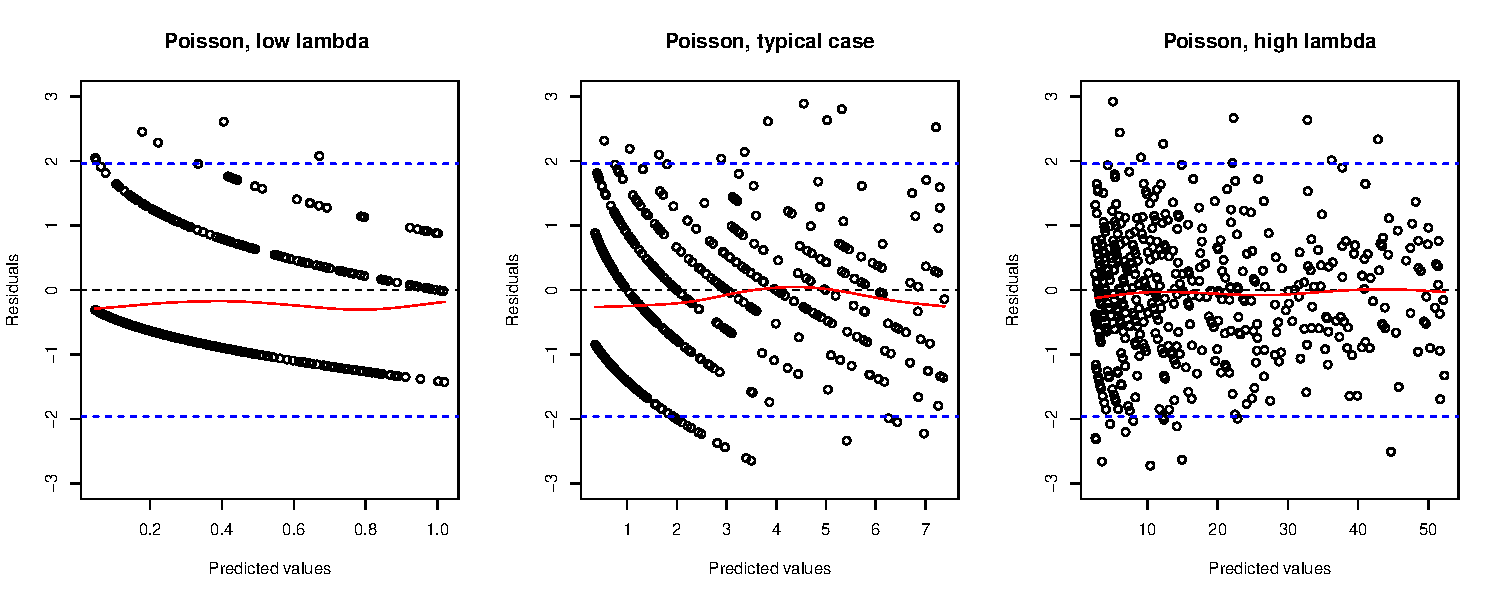
\includegraphics[width=0.9\linewidth]{figure/unnamed-chunk-4-1} 

\end{knitrout}
\end{center}
\caption{RvF Plots for conditional Poisson responses with different values of $\lambda$}
\end{figure}

\newpage

% =======================
\section{\underline{QQ - Normal Plot}}
% =======================

Before discussing how qq-normal plots of the residuals for a GLM look like, it is perhaps useful to see how they help us identify the features of a distribution. In the next figure, we display the qqnorm plots for different types of distributions. 

\begin{figure}[h!]
\begin{center}

  \begin{subfigure}[b]{0.28\textwidth}
\begin{knitrout}
\definecolor{shadecolor}{rgb}{0.969, 0.969, 0.969}\color{fgcolor}

\includegraphics[width=0.9\linewidth]{figure/unnamed-chunk-6-1} 

\end{knitrout}
  \caption{Standard Normal}
  \end{subfigure}
  \begin{subfigure}[b]{0.28\textwidth}
\begin{knitrout}
\definecolor{shadecolor}{rgb}{0.969, 0.969, 0.969}\color{fgcolor}

\includegraphics[width=0.9\linewidth]{figure/unnamed-chunk-7-1} 

\end{knitrout}
  \caption{Normal}
  \end{subfigure}
  \begin{subfigure}[b]{0.28\textwidth}
\begin{knitrout}
\definecolor{shadecolor}{rgb}{0.969, 0.969, 0.969}\color{fgcolor}

\includegraphics[width=0.9\linewidth]{figure/unnamed-chunk-8-1} 

\end{knitrout}
  \caption{Fat Tailed}
  \end{subfigure}
  
  \begin{subfigure}[b]{0.28\textwidth}
\begin{knitrout}
\definecolor{shadecolor}{rgb}{0.969, 0.969, 0.969}\color{fgcolor}

\includegraphics[width=0.9\linewidth]{figure/unnamed-chunk-9-1} 

\end{knitrout}
  \caption{Right-Skewed}
  \end{subfigure}
  \begin{subfigure}[b]{0.28\textwidth}
\begin{knitrout}
\definecolor{shadecolor}{rgb}{0.969, 0.969, 0.969}\color{fgcolor}

\includegraphics[width=0.9\linewidth]{figure/unnamed-chunk-10-1} 

\end{knitrout}
  \caption{Left Skewness}
  \end{subfigure}
  \begin{subfigure}[b]{0.28\textwidth}
\begin{knitrout}
\definecolor{shadecolor}{rgb}{0.969, 0.969, 0.969}\color{fgcolor}

\includegraphics[width=0.9\linewidth]{figure/unnamed-chunk-11-1} 

\end{knitrout}
  \caption{Bimodality}
  \end{subfigure}
\end{center}
\caption{Different types of distributions and their qq-normal plots}
\end{figure}

\begin{enumerate}
\item \emph{Standardized Normal} : Quantiles are aligned on the identity line. 
\item \emph{Normal Distribution} : Quantiles are aligned yet deviated with respect to the identity line. However, they are aligned along a line that passes through the first and the third quartiles. 
\item \emph{Fat Tails} : Quantiles in the extremes of the distribution are deviated from the line passing through the first and third quartiles, yet the rest are aligned.
\item \emph{Right Skewed} : Quantiles form the shape of a "u".
\item \emph{Left Skewed} : Quantiles form the shape of an inverted "u".
\item \emph{Bimodality} : The quantiles form the shape of an "s". 
\end{enumerate}

% -----------------------
\subsection{\underline{Standardized Residuals}}
% -----------------------

In the Normal Linear Model, residuals follow a Student's t distribution. Asymptotically, they behave normally. This can be assessed in the standard normal qq-plot.  

\begin{figure}[h]
\begin{center}
\begin{knitrout}
\definecolor{shadecolor}{rgb}{0.969, 0.969, 0.969}\color{fgcolor}
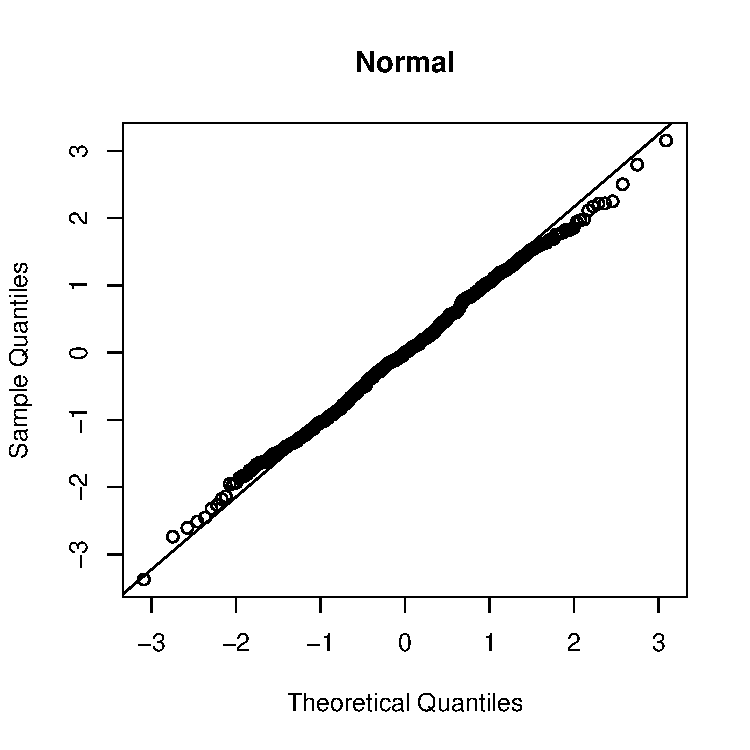
\includegraphics[width=.4\linewidth]{figure/unnamed-chunk-12-1} 

\end{knitrout}
\end{center}
\end{figure}

In the bernoulli case, deviance standardized residuals display bimodality. However, as soon as the number of trials $m_i$ starts to grow, they start becoming more and more normally distributed. An illustration of this behaviour can be seen in the next plot. 
\begin{figure}[h]
\begin{center}
\begin{knitrout}
\definecolor{shadecolor}{rgb}{0.969, 0.969, 0.969}\color{fgcolor}

\includegraphics[width=0.9\linewidth]{figure/unnamed-chunk-13-1} 

\end{knitrout}
\end{center}
\caption{qq-norm plots for Binomial GLM.}
\end{figure}

For the Poisson response, there is a concentration of negative residuals given the fact that the support of the Poisson distribution doesn't allow negative values yielding deviations on the lower quantiles from the \texttt{qqline} forming a sort of \emph{elbow} in the \texttt{qqnorm} plot. When the number of modalities starts increasing, the residuals accomodate better the standard normal distribution, as seen in the plots above. 
\begin{figure}
\begin{center}
\begin{knitrout}
\definecolor{shadecolor}{rgb}{0.969, 0.969, 0.969}\color{fgcolor}
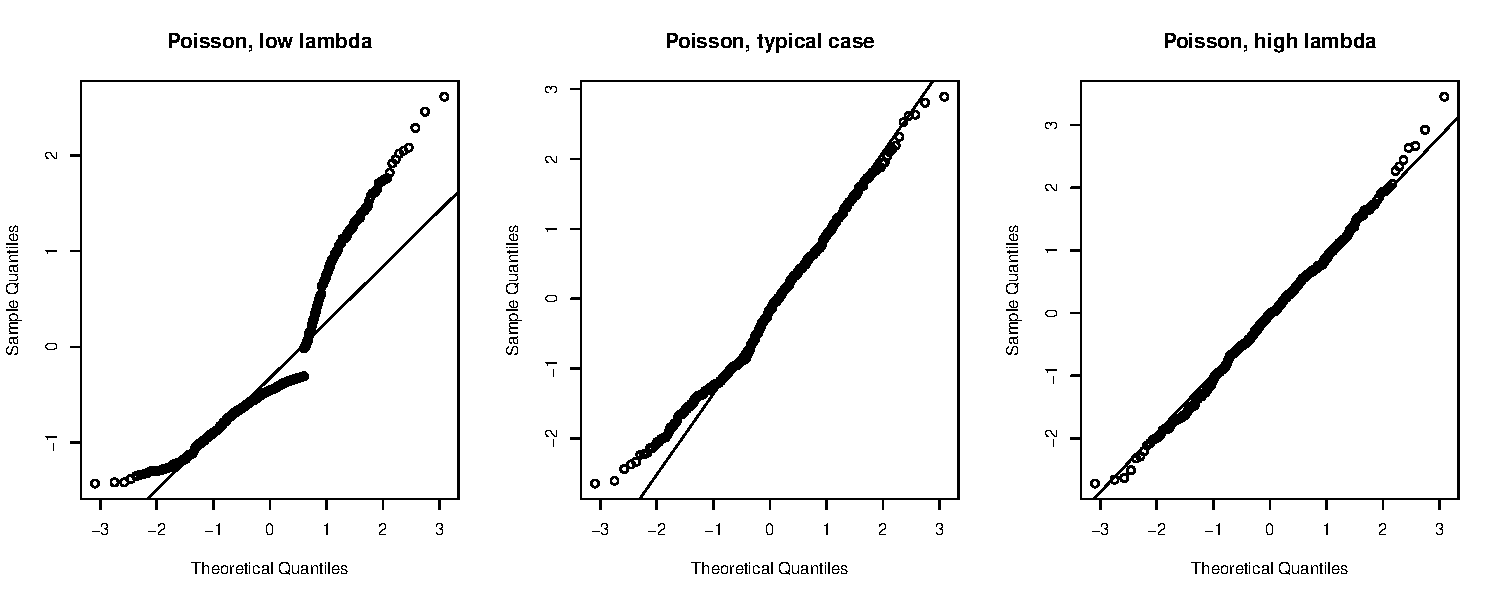
\includegraphics[width=0.9\linewidth]{figure/unnamed-chunk-14-1} 

\end{knitrout}
\end{center}
\caption{qq-norm plots for Poisson GLM.}
\end{figure}

% -----------------------
\subsection{\underline{Randomized Quantile Residuals}}
% -----------------------

An alternative way of checking model fit via residual analysis comes in the form of the qqnorm plots of randomized quantile residuals (RQ). For a continuous response (e.g. Gamma, Normal, etc.), these residuals are defined using the cdf of the responses conditioned on the fitted values denoted by $F()$. 

\begin{equation}
r_i^Q = \Phi^{-1} \oc F\op y_i ; \hat{\mu},\hat{\phi} \cp  \cc
\end{equation}

As pointed out in the class and the original paper, in presence of a discrete response, it is possible to obtain a randomized version of these residuals by setting : 
\begin{equation}
r_i^{RQ} = \Phi^{-1} \op u_i \cp \ \textrm{with: } \  u_i \sim \mathcal{U}\op \lim_{y \rightarrow y_i} F\op y ; \hat{\mu},\hat{\phi} \cp ; F\op y_i ; \hat{\mu},\hat{\phi}\cp \cc
\end{equation}

By construction, these residuals follow a normal distribution (aside from the randomness implied by $\hat{\mu}$ and $\hat{\phi}$). Moreover, in presence of a discrete response, it is necessary to check many possible realizations of the RQ residuals in order to draw conclusions. 

As it is apparent in the next plots, RQ residuals are approximately normal when the correct model is assumed. This is regardless of the number of modalities of the response. 
\begin{figure}[h]
\begin{center}
\begin{knitrout}
\definecolor{shadecolor}{rgb}{0.969, 0.969, 0.969}\color{fgcolor}
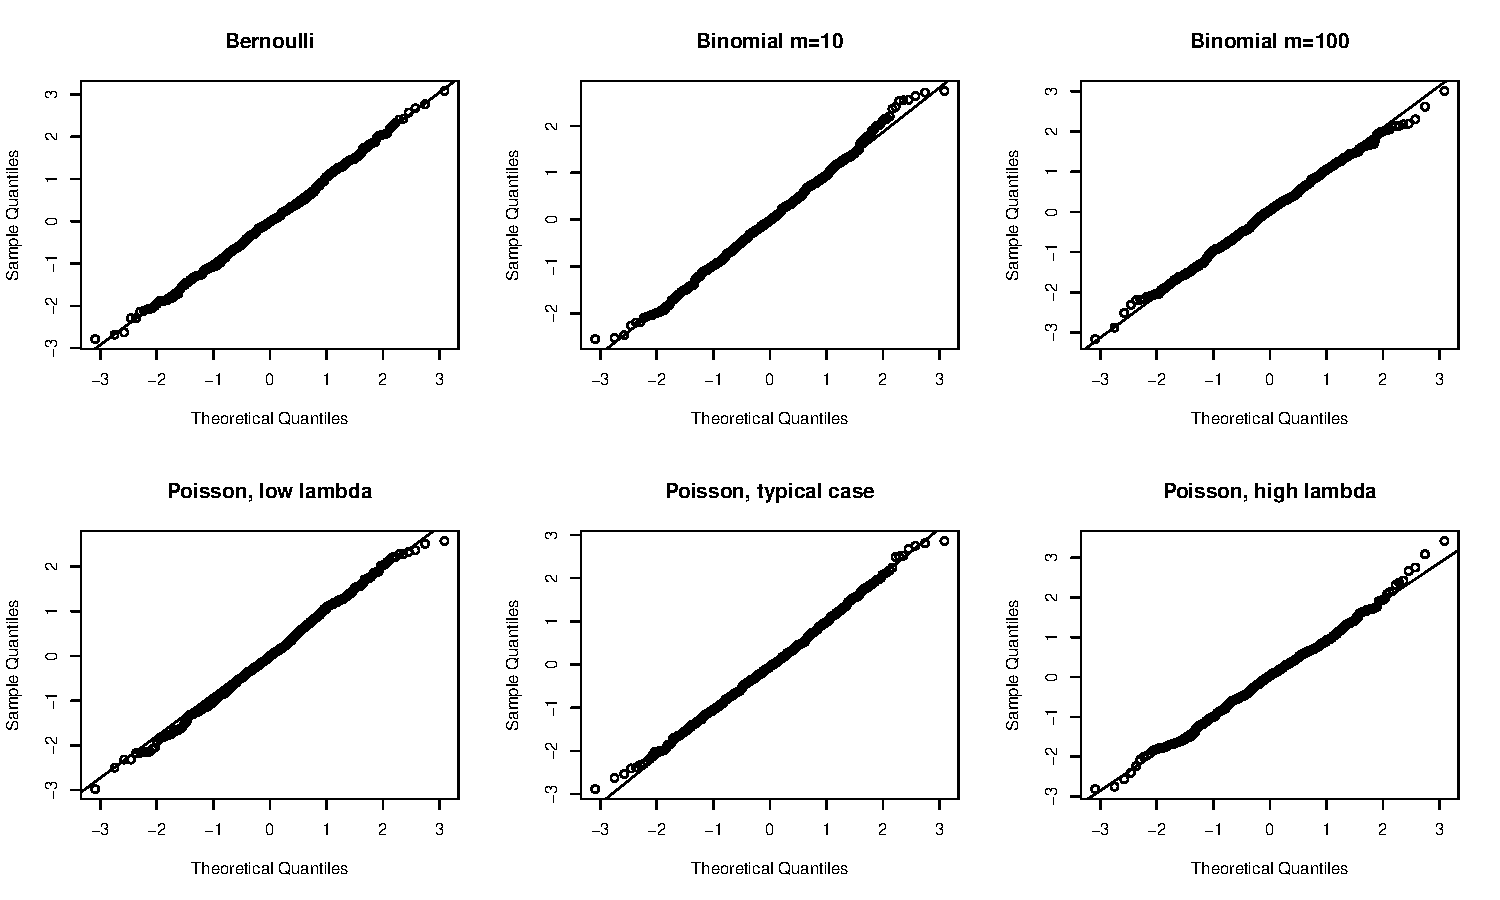
\includegraphics[width=0.9\linewidth]{figure/unnamed-chunk-15-1} 

\end{knitrout}
\end{center}
\caption{qq-norm plots for RQ residuals for Bernoulli and Poisson GLM.}
\end{figure}


% =======================
\section{\underline{Residuals vs Leverage}}
% =======================

It is known that inference on the typical GLM could be very influenced by outlying observations. These type of observations fall into two categories, working often in conjunction: 
\begin{enumerate}
  \item \emph{Points with high Residuals} : As pointed out in class, these are points for which the fitted expectation misrepresent the value of $y$. 
  \item \emph{Points with high Leverage} :  These are observations whose values of the covariates lie far in the space of their possible values. In short, they can be identified via the diagonal elements of the \emph{hat} matrix 
  \begin{equation}\mathbf{H} = \bX\op\bX^T\bX\cp^{-1}\bX^T \label{eq:hatmatrix} \end{equation} 
\end{enumerate}

In the following plot, we illustrate this influence in the linear model context with only one covariate. As it is apparent, points with high residual \emph{pull} or \emph{push} the fitted regression line, while points with high leverage and an important residual tend to have a \emph{lever} effect on the regression line. In order to identify outlying observations it is useful to check a plot of Pearson residuals vs. leverage. These plots display the Cook's distance contours as well, which allowing easier identification of points with high residuals. On the x-axis, they display the leverage score $H_{ii}$. The last plot shows that a potentially outlying observation with high leverage score can be identified by lying outside the contours for a Cook's distance of 1. 

\begin{figure}[h]
\begin{center}
\begin{knitrout}
\definecolor{shadecolor}{rgb}{0.969, 0.969, 0.969}\color{fgcolor}
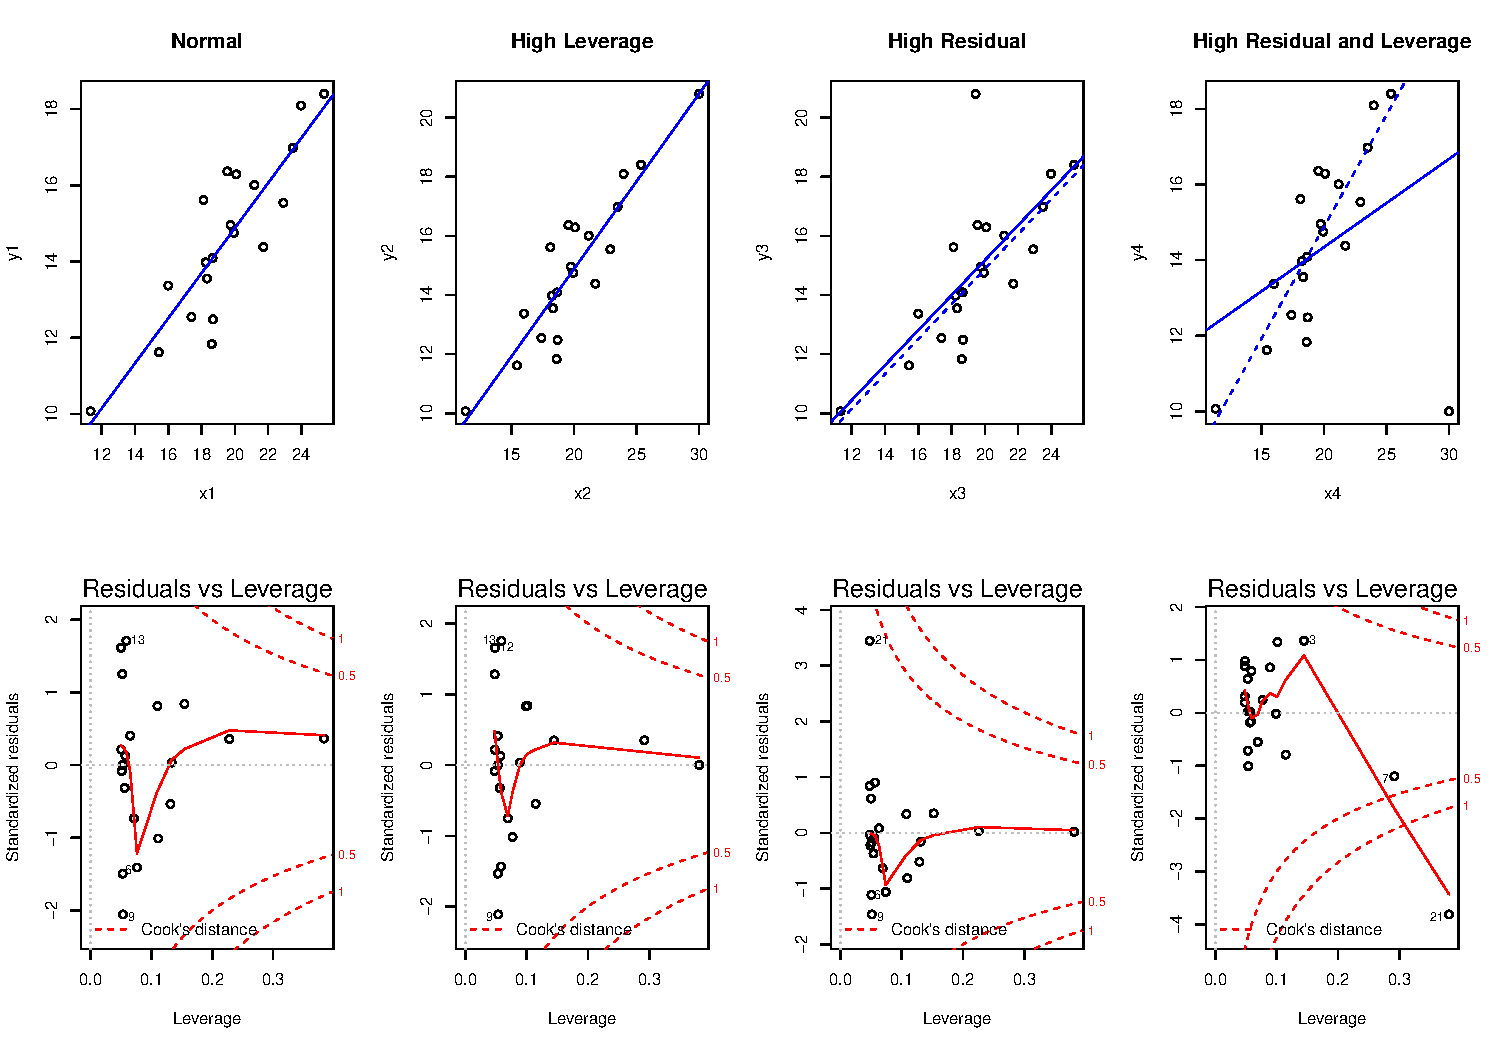
\includegraphics[width=.95\textwidth]{figure/unnamed-chunk-16-1} 

\end{knitrout}
\end{center}
\caption{Leverage, Residuals and their effect on estimation for a linear model.}
\end{figure}

The conclusions drawn from this type of plots are valid in the GLM context with the usual definition of the Pearson Residuals in \eqref{eq:pearsonres} and the leverage scores obtained via the \emph{hat} matrix defined in \eqref{eq:hatmatrix}.

\end{document}
